
\subsubsection{Datenbanklayout}
Da die Anzahl der Datentypen in SQLite auf NULL, INTEGER, REAL, TEXT und BLOB beschränkt ist, \url{http://www.sqlite.org/datatype3.html}, ist das Datenbankschema von Warranty schnell definiert.
\newline
Um die Einzigartigkeit der Einträge zu gewährleisten, ist die ID als auto- increment gekennzeichnet. Somit können wir sicherstellen, dass auch IDs von gelöschten Einträgen nicht wiederverwendet werden. 
\newline
Da SQLite keine Datentypen für Datum und Zeit zur Verfügung stellt, wir aber trotzdem Datumsstempel benötigen, greifen wir auf den Datentyp TEXT und Datumsfunktionen wie „date“ von SQLite zurück \url{http://www.sqlite.org/lang_datefunc.html}.
\newline
\begin{figure}[h]
\centering
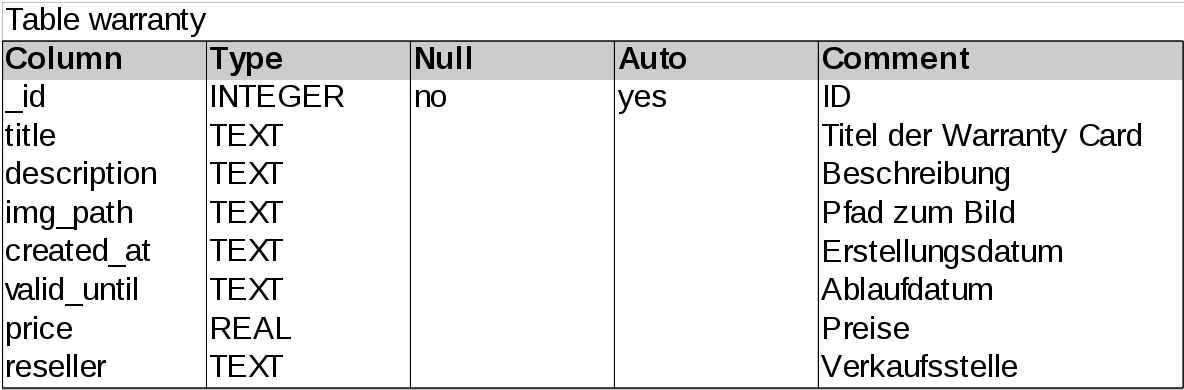
\includegraphics[height=5cm]{sqlitetbl_warranty.png} \\
\caption{Datenbankschema Tabelle Warranty}
\end{figure}

Der einzige Index liegt auf der ID, da in der App sämtliche Aktionen mittels dieser ID als Referenz ausgeführt werden. Da wir keine Volltextsuche implementiert haben, benötigen wir kein weiteren Indizes.
\begin{figure}[h]
\centering
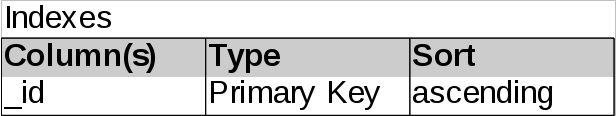
\includegraphics[height=1.5cm]{sqliteidx_warranty.png} \\
\caption{Datenbankschema Tabelle Warranty}
\end{figure}

\subsubsection{Datenbank erstellen}
Ist das Datenbankschema definiert, ist die Implementierung in der App eine kleine Sache. Zuerst werden die Attribute benannt. Wachsamen Lesern fällt auf, dass sämtliche Strings „public static final“ sind. Dies erlaubt es den Programmierern, von überall her dynamisch auf die Namen der Attribute zuzugreifen, sodass bei einer allfälligen Anpassung des Schemas immer die korrekten Namen in den SQL Statements verwendet werden.
\newline

\begin{lstlisting}[caption=Attributdeklaration,captionpos=b,lang=java]
public class TBLWarrantyHelper extends SQLiteOpenHelper {
	public static final String TBL_NAME="warranty";
	public static final String CLMN_ID = "_id";
	public static final String CLMN_TITLE = "title";
	public static final String CLMN_DESC = "description";
	public static final String CLMN_IMGPATH = "img_path";
	public static final String CLMN_CREATEDAT = "created_at";
	public static final String CLMN_VLDTIL = "valid_until";
	public static final String CLMN_PRICE = "price";
	public static final String CLMN_RESSELLER = "reseller";
\end{lstlisting}
Anschliessend wird das Creation- Statement der Tabelle mit den dazugehörigen Datentypen vorbereitet.

\begin{lstlisting}[caption=Tabellen Creation Statement,captionpos=b,lang=java]
	private static final String DB_CREATE="create table " + TBL_NAME + " (" +
		CLMN_ID + " integer primary key autoincrement," + 
		CLMN_TITLE + " text," + 
		CLMN_DESC + " text," + 
		CLMN_IMGPATH + " text," + 
		CLMN_CREATEDAT + " text," +
		CLMN_VLDTIL + " text," +
		CLMN_PRICE + " real," +
		CLMN_RESSELLER + " text);";
\end{lstlisting}

Zum Schluss wir die von SQLiteOpenHelper [Glossar] geerbte Methode onCreate(SQLiteDatabase db) überschrieben und darin das Statement als SQL ausgeführt.
\begin{lstlisting}[caption=SQL Statement,captionpos=b,lang=java]
	@Override
	public void onCreate(SQLiteDatabase db) {
		db.execSQL(DB_CREATE);
	}
\end{lstlisting}

\subsubsection{Insert und Update}
Die aus Anwendersicht vermutlich wichtigsten Methoden sind die Insert- und die Update- Methoden. Da diese von der Funktionalität sehr ähnlich sind, ist aus Sicht des Programmierers sinnvoll, diese zusammen zulegen. Der grundlegende Unterschied ist , dass beim Insert ein neuer Eintrag erstellt, beim Update ein bereits vorhandener Eintrag angepasst wird.

Im Javacode ist die Differenzierung denkbar einfach.
\begin{lstlisting}[caption=Tabellen Creation Statement,captionpos=b,lang=java]
public void insertWarrantyCard(WarrantyCard card){
	...
	if (card.get_id() == 0) {
		db.insert(TBLWarrantyHelper.TBL_NAME, null, values);
	} else {
		db.update(TBLWarrantyHelper.TBL_NAME, values, TBLWarrantyHelper.CLMN_ID + "=" + card.get_id(), null);
	...
	}
\end{lstlisting}
Der Grund für diese einfache Unterscheidung liegt in der Auflistung der Quittungen im Homescreen [Glossar] der App. Diese sogenannte Listview [Glossar] kennt von jeder aufgelisteten Quittung ihre dazugehörige ID. Möchte der User eine Quittung bearbeiten, wird in der App intern diese Referenz auf die Quittung weitergegeben. Möchte der User eine neue Quittung hinterlegen, wird das ID Feld nicht gefüllt. Dies führt dazu, dass der Standard Integer- Wert, in Java eine 0, weitergegeben wird. \url{http://docs.oracle.com/javase/tutorial/java/nutsandbolts/datatypes.html}


\subsubsection{Delete}
Da die Quittungen nach deren Ablauf nicht automatisch gelöscht werden, kann es durchaus sein, dass ein User die Quittungen manuell löschen möchte. 
Wie bereits im Kapitel „Insert und Update“ erwähnt, ist der Listview auf dem Homescreen die ID jeder aufgelisteten Quittung bekannt. Somit kann eine Quittung direkt aus der Listview mit dem Methodenaufruf deleteCard und der dazugehörigen ID, die anschliessend das entsprechende SQL- Statement an die Datenbank kommuniziert, gelöscht werden.
\newline
Wie bereits beim Insert und Update haben wir uns auch hier die Tatsache, dass das auto increment von SQLite bei eins beginnt zu nutzen gemacht. Wird null als ID übergeben, hat dies zur Folge, dass ausnahmslos alle gespeicherten Quittungen gelöscht werden.

\begin{lstlisting}[caption=deleteCard Methode,captionpos=b,lang=java]
public void deleteCard(int cardID) {
	...
	if (cardID == 0) {
		db.delete(TBLWarrantyHelper.TBL_NAME, null, null);
	} else {
		db.delete(TBLWarrantyHelper.TBL_NAME, TBLWarrantyHelper.CLMN_ID + "=" + cardID, null);
	}
	...
}
\end{lstlisting}
Eine Funktion zum löschen aller Quittungen wurde im Menü des Homescreens untergebracht.